\documentclass[letterpaper,11pt]{article}
\usepackage{mystyle}

% Uncomment this section if you wish to have a header.
%\usepackage{fancyhdr} 
%\pagestyle{fancy} 
%\renewcommand{\headrulewidth}{0.5pt} % customise the layout... 
%\lhead{} \chead{<++>} \rhead{<++>} 
%\lfoot{} \cfoot{\thepage} \rfoot{}


\begin{document}
\title{A Graph Parallel Implementation of Hidden Markov Models}
\author{Kevin Schmid, Andy Shi, Ding Zhou \\ CS 205 \\
Harvard College \\ Cambridge, MA}
\date{May 11, 2015}
\maketitle

% No indentation for new paragraphs
%\setlength\parindent{0pt}

% Skip a line between paragraphs
%\setlength\parskip{2ex}

% Put your stuff here

\begin{abstract}
    Put abstract here

\end{abstract}

\begin{multicols*}{2}

\section{Introduction}

Hidden Markov models (HMM) are often used to model time-series data for both
discrete and continuous data. HMM has been successfully applied to problems such as speech recognition \cite{hmm-speech} and gesture recognition \cite{hmm-gesture}. The
parameters to a hidden Markov models are most commonly learned from the
Baum-Welch---an Expectation Maximization (EM) algorithm. Unfortunately, the
Baum-Welch algorithm is quadratic in number of states. A parallel implementation
of the EM algorithm along the state axis would greatly improve scalability.
Graph based platforms are particularly suited to EM algorithms, and our project
uses GraphLab~\cite{graphlab}, a platform created by Dato~\cite{dato} for implementing graph based parallelizing schemes. 

Our code is available at
\url{https://github.com/cs205-project-group/hmm}.


\section{Background}

\subsection{Hidden Markov Model}
A hidden Markov model assumes that the system follows a Markov process. For this paper, we will assume a finite number of states and observations. The probability of transitioning from state $i$ to state $j$ only depends on the current state, and we define transition matrix $A$ such that element $a_{ij}$ is the probability  of transitioning from $i$ to $j$. In an HMM, we cannot observe states, but we can observe outputs generated by the states. Given $N$ states and $M$ observations, we capture this with a $N \times M$ emission matrix $B$, where $b_{ij}$ is the probability of observation $j$ given the state is $i$. Finally, we define a $N$ length vector as $\pi$ as the prior, where $\pi_i$ is the probability of initial state being $i$. 

We can thus capture all the information about an HMM with $\theta = (A, B, \pi)$. In an HMM, we are given a sequence of $T$ observations, and we will use a series of forward and backwards propagations to estimate the parameters $\theta = (A, B, \pi)$.

\subsection{Baum-Welch}

The following explanation is based on Wikipedia's presentation of the algorithm. \cite{bwwiki}

Let $(X_1, X_2, \ldots, X_N)$ denote the $N$ states and $\bold{O} = \{O_1, O_2, \ldots, O_T\}$ the $T$ observed outputs. The Baum-Welch algorithm uses expectation-maximization to find the maximum likelihood estimate.

Suppose we begin with some initial parameters, $\theta  =  (A, B, \pi)$.  Given the observation sequence, our task is to update these parameters based on insights from the training sequence.  

Given our training sequence, Baum-Welch first figures out the probability of being in a state at some time in the ``run" of the observation sequence.  Let's call this $\gamma_{i}(t)$, the ``probability of being in state $i$ at time $t$ of this observation sequence given our current model parameters," $P(X_t = i | \bold{O}, \theta)$.

How can we figure this out? To do this, the Baum-Welch algorithm performs two sub-calculations, for the ``forward probabilities" and the ``backward probabilities."  Like $\gamma_i(t)$ values, the forward probability are computed for each ($\textit{state}, \textit{time}$) pair: given some observation sequence and our current moel, the forward probability $\alpha_i(t)$ is the probability of seeing the observation sequence up to time $t$ and landing in state $i$.  The backward probability is defined analogously: it's the probability of starting in some state $i$ and seeing the observation sequence \textit{from} time $t$ until the end.

We can define the forward and backward probabilities recursively:

\begin{equation} \label{alpha}
\alpha_i(t+1) =  b_{jo_1}\sum_{i=1}^{N} \alpha_i(t)a_{ij}
\end{equation}

\begin{equation} \label{beta}
\beta_i(t) = \sum_{i=1}^N \beta_j(t+1)a_{ij}b_j(o_{t+1})
\end{equation}

We can put the alpha and beta probabilities together to find $\gamma_i(t)$.  Some intuition for this formula: the bottom is the probability of being in \textit{some state} at time $t$ given our \textit{entire} observation sequence.  The top is the probability of being in some particular state $i$ at time $t$ given our \textit{entire} observation sequence.  For both numerator and denominator, you have to get to the state at that time (forward probability) and leave from the state next and finish emitting the observation sequence  (backward probability).

\begin{equation} \label{gamma}
\gamma_i(t) = P(X_t = i | \bold{O}, \theta) = \frac{\alpha_i(t) \beta_i(t)}{\sum_{j=1}^N \alpha_j(t) \beta_j(t)}
\end{equation}

From here, we can figure out our updates for the $B$ matrix and the new prior. 

$B$ can be updated by: 
\begin{equation}\label{b}
b^*_{i,v_k} = \frac{\sum_{t=1}^{T}1_{o_t = v_k} \gamma_i(t)}{\sum_{t=1}^T \gamma_i(t)}
\end{equation}
where $1_{o_t = v_k}$ is $1$ if $o_t = v_k$ and $0$ otherwise. 

Intuition: the update for  $b^*_{i,v_k}$ is just the frequency across the entire observation sequence of being in the state $i$ and seeing $v_k$.

\begin{equation}\label{pi}
\pi_i^* = \gamma_i(0)
\end{equation}

Intuition: this is the probability of being in state $i$ before the observation sequence begins.  

To update the $A$ matrix (each $a_{ij}$ entry), we need to figure  out the probability of being in state $i$ and $\textit{moving}$ to state $j$ next.  Fortunately, this calculation can be done in a straightforward way, and we can think of it as a ``relative frequency calculation" of the transitions that begin at state $i$ and go to state $j$ compared to the transitions through state $i$.  This ``relative frequency intuition" is provided by \cite{rabiner1986introduction}.

Define $\xi_{ij}(t)$ to be the probability of being in state $i$ at time $t$ and state $j$ at time $t+1$ given $\bold{O}$ and parameter $\theta$. 
\begin{equation}\label{xi}
\begin{aligned}
\xi_{ij}(t) &= P(X_t = i, X_{t+1} = j | \bold{O}, \theta)  \\
&=\frac{\alpha_i(t) a_{ij} \beta_j(t+1)b_{jo_{t+1}}}{\sum_{k=1}^N \alpha_k(t) \beta_k(t)}
\end{aligned}
\end{equation}
Finally, $A$ can be updated by: 

\begin{equation}\label{a}
a^*_{ij} = \frac{\sum_{t=1}^{T-1}\xi_{ij}(t)}{\sum_{t=1}^{T-1}\gamma_i(t)}
\end{equation}

These steps are repeated until the parameters converge. 

\subsection{Prior Work}

Here we review prior work related to \textit{parallelization} of hidden Markov models specifically.  In 2009, Chuan Liu conducted an independent project aiming to implement HMM training in parallel on CUDA.  The project's parallelization of the  forward-backward probabilities computation informed how we could approach parallelizing this part, even though our representation in our framework ended up distinctively graph-based.  The rest of his work frames computations in terms of matrix multiplication operations.  His work also utilizes ``parallel reduction" for computing the sum of a vector, something we've seen in CS205.  \cite{cuda-hmm}

Also, we noted the approach of Li et. al in 2010, applying an earlier parallelization approach - ``cut and stitch" - to the problem of hidden Markov model training.  The ``cut and stitch" approach parallelizes along the length of the input observation sequence (along the $T$-axis).  The graph parallel scheme in this paper is orthogonal to the ``cut and stitch" approach, and we are excited about the prospect of applying these two parallelization schemes to the problem of HMM training. \cite{cut-stitch}

\section{System Description}

We benchmarked our code on the Odyssey cluster, supported by the FAS Division of
Science, Research Computing Group at Harvard University~\cite{odyssey}.


\section{Performance Evaluation}

We evaluated the performance of our code, measuring runtime of our serial and
graph parallel code for a variety of $N$, $M$, and $T$. We generated synthetic
data with random $(A, B, \pi)$ as the true parameters, and initialized our
Baum-Welch training parameters randomly. For both the serial and parallel
versions, we ran 5 update iterations of the Baum-Welch algorithm.  Additionally,
we also varied the number of cores available for GraphLab. R~\cite{r} was used
for data analysis and plotting. 

Our parallel code's runtime, compared to that of the serial version, is shown in
Figure~\ref{fig:runtime-256-500}. We see that, while our GraphLab implementation
runs slower than our serial implementation, the running time still decreases as
we increase the number of processing cores. 

\begin{figure*}[htb]
    \centering
    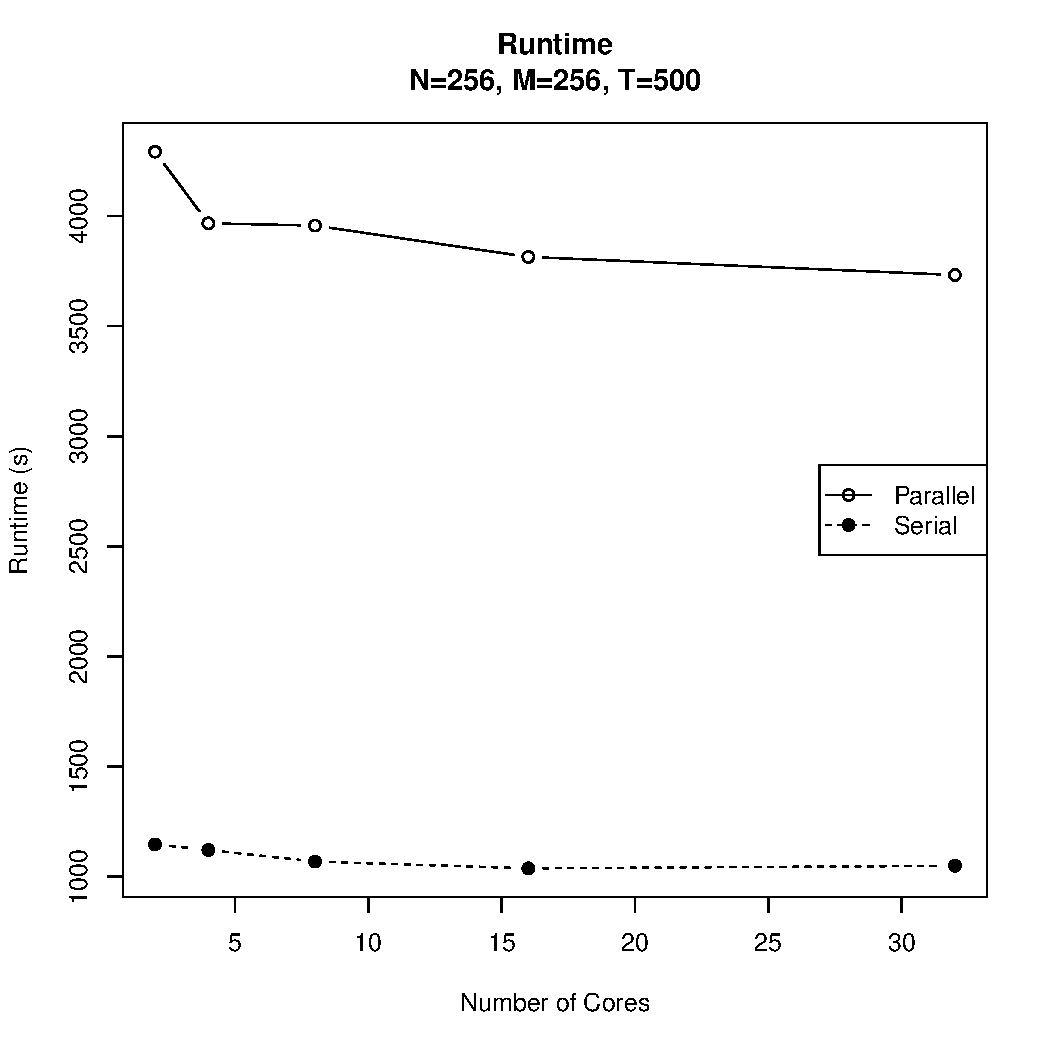
\includegraphics[width=0.6\textwidth]{../figure/runtime-N_256-T_500.pdf}
    \caption{Runtime as a function of number of cores used.}
    \label{fig:runtime-256-500}
\end{figure*}

Figures for other testing conditions are shown in the appendix, in
Figures~\ref{fig:runtime1}--\ref{fig:runtime4}. In general, runtime for the
serial code remains constant, and runtime for the parallel code decreases with
more processors. In many cases, runtime increases when going from 2 to 4
cores---this may represent increased communication cost between more processors.
Noise in our plots may be caused by changes in processing load on the Odyssey
server.

We examined how our implementation scales as we increase the
problem size, especially $N$. A log-log plot of running time vs. $N$ is shown in
Figure~\ref{fig:scaling-16-200}. Judging by the slopes on the graph, our
GraphLab code scales better than the serial code for smaller $N$, but unfortunately not for other values of $N$. 

\begin{figure*}[htb]
    \centering
    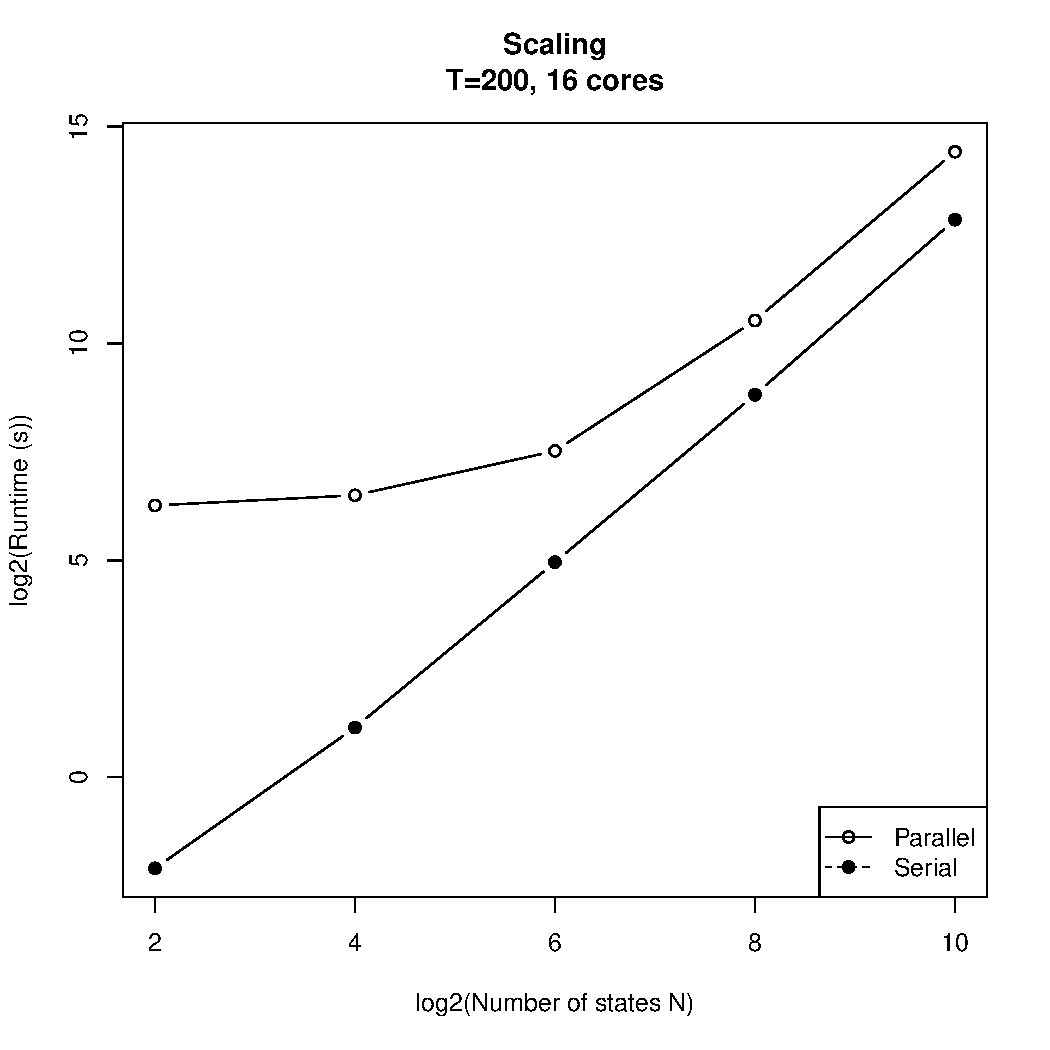
\includegraphics[width=0.6\textwidth]{../figure/scaling-cores_16-T_200.pdf}
    \caption{Log-Log plot of runtime as a function of number of states $N$.}
    \label{fig:scaling-16-200}
\end{figure*}

Additional figures for other testing conditions display similar trends and are
shown in the appendix, Figures~\ref{fig:scaling1}--\ref{fig:scaling4}. 


\section{Conclusion}

Our implementation is awesome



\end{multicols*}

\end{document}
